\documentclass[11pt]{article}
\usepackage{tikz}
\usepackage{forloop}
\usetikzlibrary{shadows, arrows}

% Define block styles
\tikzstyle{block} = [draw, fill=blue!20, text width=6.0em, text centered, minimum height=1.5em, drop shadow]
\tikzstyle{layer} = [block, text width=10em, minimum width=14em, minimum height=3em, rounded corners, drop shadow]
\tikzstyle{line} = [draw, thick, color=black!90, -latex']

% Draw layer
\newcommand{\layer}[2]{
node (l#1) [layer] {#2}}

\newcommand{\arrow}[4]{
  \path [line] (#1.south) -- node [right]
    {#3, #4} (#2);}

\begin{document}
	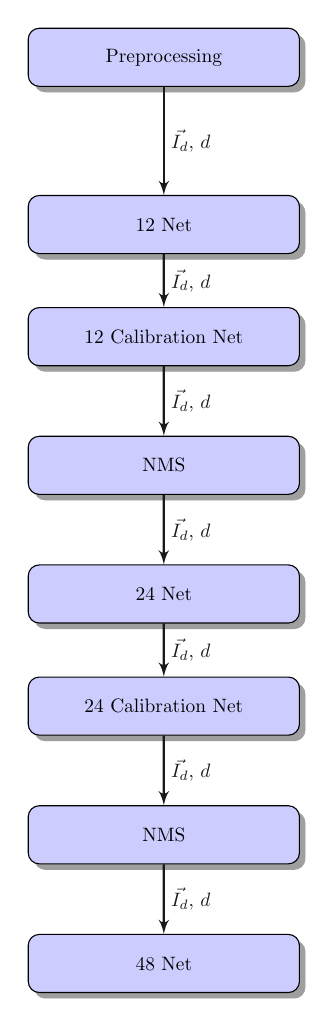
\begin{tikzpicture}[scale=0.7, transform shape]
		
		% Draw diagram elements
		\path \layer{1}{Preprocessing};
		\path (l1.south)+(0.0, -2.5) \layer{2}{12 Net};
		\path (l2.south)+(0.0, -1.5) \layer{3}{12 Calibration Net};
		\path (l3.south)+(0.0, -1.8) \layer{4}{NMS};
		\path (l4.south)+(0.0, -1.8) \layer{5}{24 Net};
		\path (l5.south)+(0.0, -1.5) \layer{6}{24 Calibration Net};
		\path (l6.south)+(0.0, -1.8) \layer{7}{NMS};
		\path (l7.south)+(0.0, -1.8) \layer{8}{48 Net};
		
		% Draw arrows between elements
		\arrow{l1}{l2}{$\vec{I_d}$}{$d$};
		\arrow{l2}{l3}{$\vec{I_d}$}{$d$};
		\arrow{l3}{l4}{$\vec{I_d}$}{$d$};
		\arrow{l4}{l5}{$\vec{I_d}$}{$d$};
		\arrow{l5}{l6}{$\vec{I_d}$}{$d$};
		\arrow{l6}{l7}{$\vec{I_d}$}{$d$};
		\arrow{l7}{l8}{$\vec{I_d}$}{$d$};
		
	\end{tikzpicture}
\end{document}
